%%%%%%%%%%%%%%%%%%%%%%%%%%%%%%%%%%%%%%%%%%%%%%%%%%%%%%%%%%%%%%%
%
% Welcome to Overleaf --- just edit your LaTeX on the left,
% and we'll compile it for you on the right. If you open the
% 'Share' menu, you can invite other users to edit at the same
% time. See www.overleaf.com/learn for more info. Enjoy!
%
%%%%%%%%%%%%%%%%%%%%%%%%%%%%%%%%%%%%%%%%%%%%%%%%%%%%%%%%%%%%%%%
\documentclass{beamer}


\hypersetup{
    colorlinks=true,
    linkcolor=blue,
    filecolor=magenta,      
    urlcolor=magenta,
    citecolor=blue!60!black}
\usepackage[english]{babel}
%\usepackage{biblatex}
\usepackage[backend=biber, style=apa]{biblatex}
\addbibresource{references.bib}
\usepackage{booktabs}
\usepackage{svg}
\usepackage{graphicx}
\usepackage{listings}
\lstset{language=Python,basicstyle=\ttfamily,keywordstyle=\color{blue}}

%Information to be included in the title page:
\title{A Step Towards Explainable AI: Learning a Natural Language Processing Model to Reason Like a Taxonomist}
\author{Robert van de Vlasakker}
\institute{Wageningen University \& Research}
\date{07-02-2022}

\begin{document}
\graphicspath{ {./figures/} }

\frame{\titlepage}

\begin{frame}
\frametitle{Binary Classifier for Descriptions}
\begin{figure} [htbp]
    \centering
    %\vspace{-2cm}
    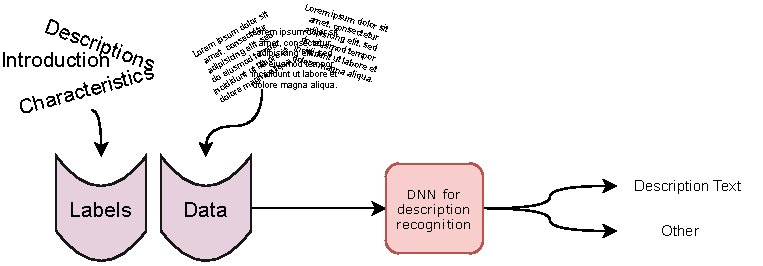
\includegraphics[width=\textwidth]{figures/midterm_explain_4.pdf}
\end{figure}
Data come from several structured sources like Wikipedia:
\begin{itemize}
    \item Text are used a features
    \item Headers are used as labels
\end{itemize}
\end{frame}


\begin{frame}
\frametitle{Part of Speech (Part 1)}
\begin{figure} [htbp]
        \centering
        %\vspace{0cm}
        \includesvg[inkscapelatex=false, width=\textwidth]{PoS_example.svg}
        %\caption[Example of part of speech tagging (1)]{An example of part of speech and dependency parsing for the sentence "The Brown bear has brown fur.". The arrows contain the dependency tags and the words contain the part of speech tags.}
        \label{fig:PoS_example}
\end{figure}
\end{frame}


\begin{frame}
\frametitle{Part of Speech (Part 2)}
\begin{figure} [htbp]
        \centering
        %\vspace{0cm}
        \includesvg[inkscapelatex=false, width=.6\textwidth]{PoS_example2.svg}
        %\caption[Example of part of speech tagging (2)]{An example of part of speech and dependency parsing for the sentence "The claws are sharp.". The arrows contain the dependency tags and the words contain the part of speech tags.}
        \label{fig:PoS_example2}
\end{figure}
\end{frame}


\begin{frame}
\frametitle{Part of Speech (Part 3)}
\begin{figure} [htbp]
        \centering
        %\vspace{-2cm}
        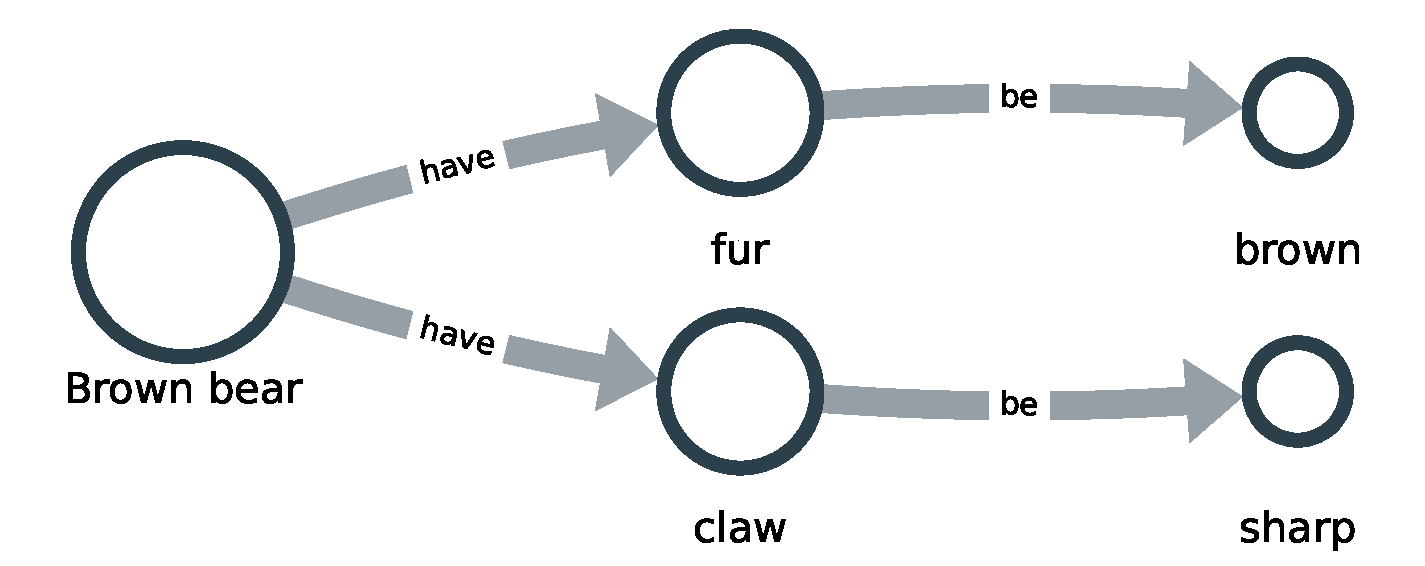
\includegraphics[width=\textwidth]{figures/kn_example_v2.pdf}
        %\caption[Example of a knowledge graph]{The sentences result in five nodes (subject/object) and four edges (relations). The circles contain the objects/subjects and the arrows represent the relations.}
        \label{fig:graph_example}    
\end{figure}
\end{frame}



{
\setbeamertemplate{background} 
{
    \hspace{5.5cm}
    \includesvg[inkscapelatex=false, height=\paperheight]{glossary_example.svg}
}
\begin{frame}
\frametitle{Botanic Glossary (part 1)}
\begin{itemize}
    \item Matching every sentence against a Botanic glossary from \href{https://en.wikipedia.org/wiki/Glossary_of_plant_morphology}{Wikipedia/glossary}
    \item Glossary contains generic and specific botanic terms
    \item Will select only relevant traits
    \item And filter out miss classified sentences
\end{itemize}
\end{frame}
}


\begin{frame}[fragile]
\frametitle{Botanic Glossary (part 2)}
Python pseudo code:

\begin{lstlisting}
glossary['roots'] = [
    'root hairs',
    'fasciculated root',
    'nodulose root',
    ...
]
glossary['roots'] = [
    'blade',
    'rachilla',
    'surface',
    ...
]
\end{lstlisting}
\end{frame}


\begin{frame}[fragile]
\frametitle{Botanic Glossary (part 3)}
\begin{lstlisting}
'The green leaves with sharp edge and 10 mm wide.'
\end{lstlisting}
apply extraction:
\begin{lstlisting}
[('species', 'has main part', 'leaves'), 
('leaves', 'has part', 'leave'), 
('leave', 'has color', 'green'), 
('leave', 'is', 'with sharp edge'), 
('leave', 'measures', '10 mm wide'),]
\end{lstlisting}
\end{frame}



\begin{frame}[fragile]
\frametitle{Species Classifier (part 1)}
Combine the triples (for now) and feed them to a classifier to extract the most important traits.

\begin{lstlisting}
[('species', 'has main part', 'leaves'), 
('leaves', 'has part', 'leave'), 
('leave', 'has color', 'green'), 
\end{lstlisting}
results in:
\begin{lstlisting}
'Species has main part leaves.'
'The leave has part leave.'
'Leave has color green''
\end{lstlisting}
\end{frame}


\begin{frame}
\frametitle{Species Classifier (part 2)}
And colorize the importance:
\begin{figure} [htbp]
    \centering
    %\vspace{-2cm}
    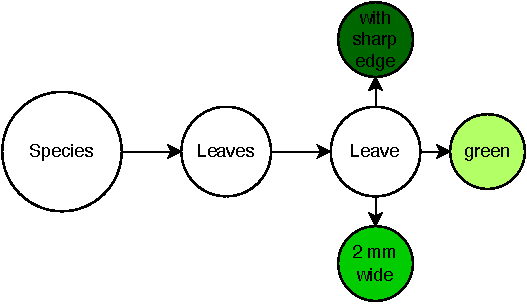
\includegraphics[width=\textwidth]{figures/plantnet_example_informationgraph.pdf}
\end{figure}
\end{frame}

\begin{frame}
\frametitle{Species Classifier (part 3)}
And can result in complex graph (working example for leaves only):
\begin{figure} [htbp]
    \centering
    %\vspace{-2cm}
    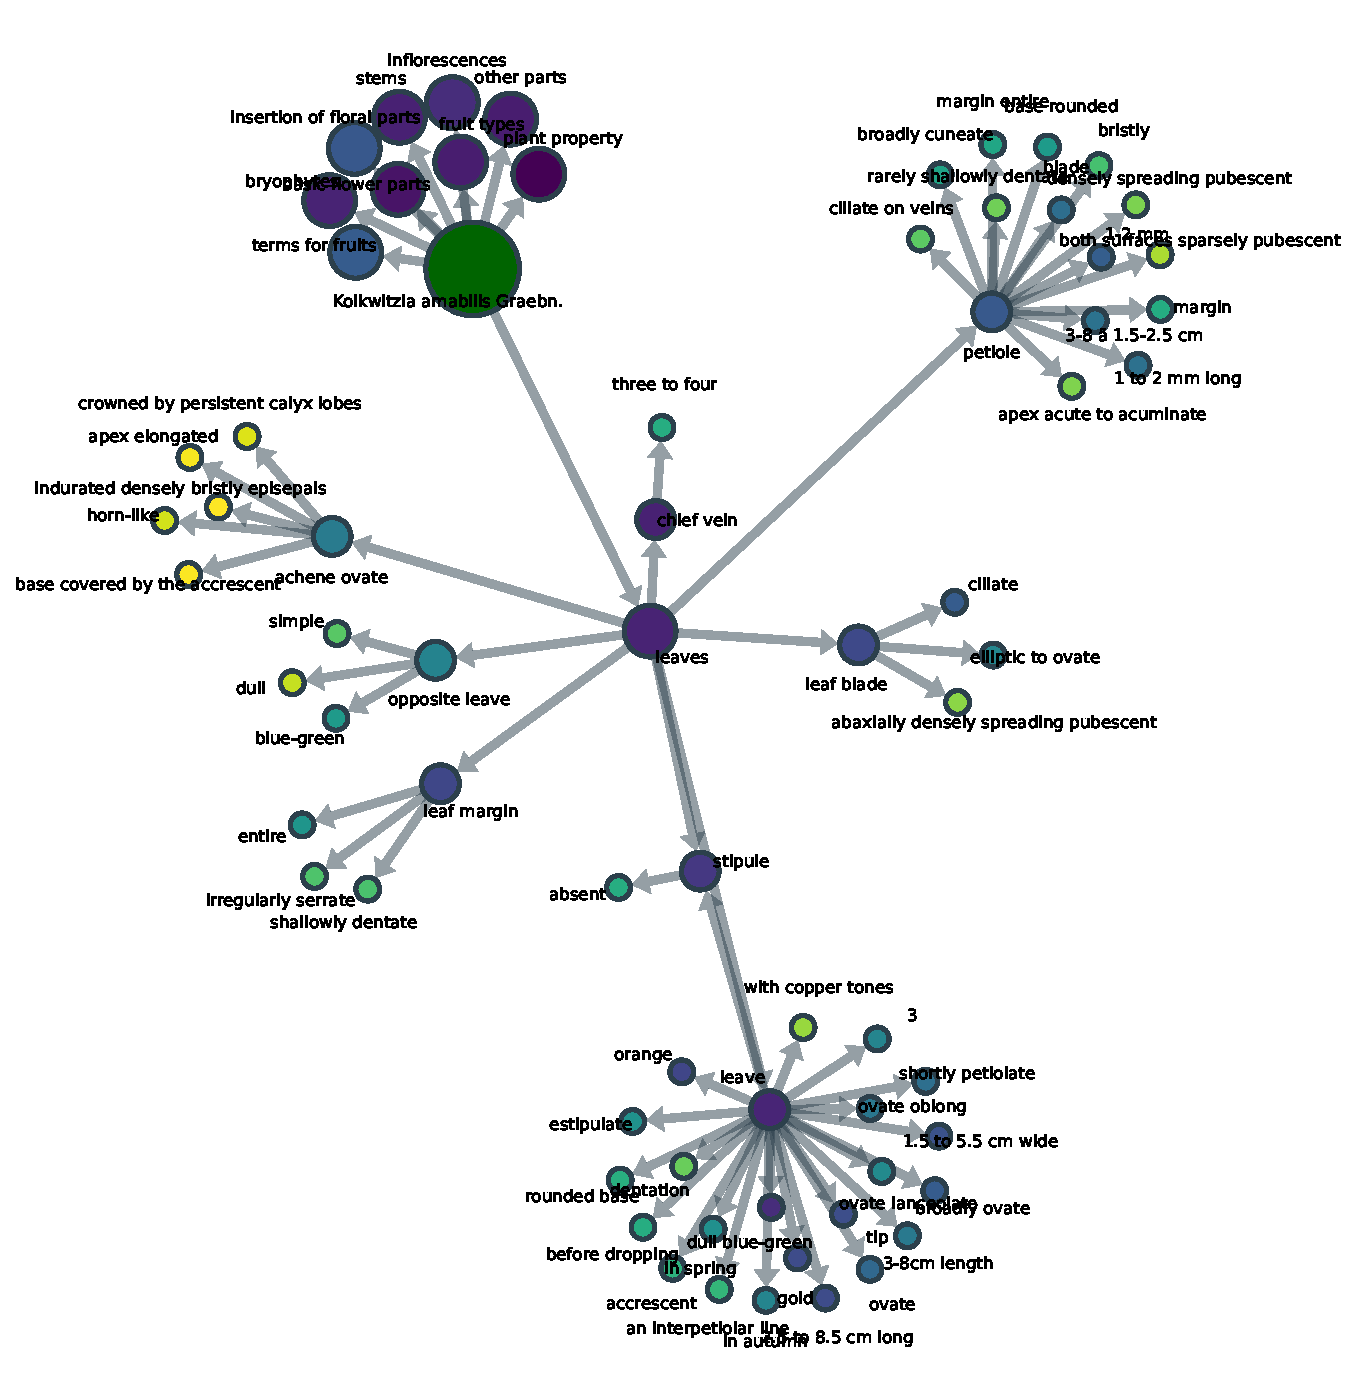
\includegraphics[width=0.7\textwidth, height=0.8\paperheight]{figures/plantnet_workingexample.pdf}
\end{figure}
\end{frame}


\begin{frame}
\frametitle{And now?}
\begin{itemize}
    \item Do the extracted traits make sense?
    \item Are yellow traits really important?
    \item Process traits further?
    \item Create dictionary counter with traits instead of text spans?
   \item Switch to graph networks?
\end{itemize}
\end{frame}


\end{document}

